\documentclass[conference]{IEEEtran}

\usepackage{graphicx}
\usepackage{amsmath, amssymb}
\usepackage{hyperref}
\usepackage{caption}
\usepackage{cite}
\usepackage{float}

\title{D.I.A.G.R.A.M.: Development of Image Analysis for Graph Recognition And Modeling}

\author{
    \IEEEauthorblockN{Filippo Garagnani, Saverio Napolitano, Nicola Ricciardi}
    \IEEEauthorblockA{
        'Computer Vision and Cognitive System' course \\
        \textit{Università di Modena e Reggio Emilia}
    }
}

\begin{document}

\maketitle

\begin{abstract}
This report describes D.I.A.G.R.A.M., a system for diagram recognition and generation. We present its architecture, the logic behind deterministic algorithms and the training of its deep learning components. The project aims to transform visual diagram input into structured representations.
\end{abstract}

\section{Introduction}
Diagrams are crucial in education, documentation, and many other fields. Developing a system that automatically understands and generates diagrams may reveal helpful for having high-quality, easily editable representations. This, however, poses challenges involving classification, shape detection, structure interpretation and symbolic representation. Our project proposes a modular architecture to tackle these tasks.

% System Architecture
\section{System Architecture}
Figure~\ref{fig:pipeline} illustrates the full pipeline, composed of four main modules: the Classifier, Extractor, Transducer, and Compiler. Each module is designed to process and transform the handwritten diagram image progressively toward a structured output.

\begin{figure}[H]
\centering
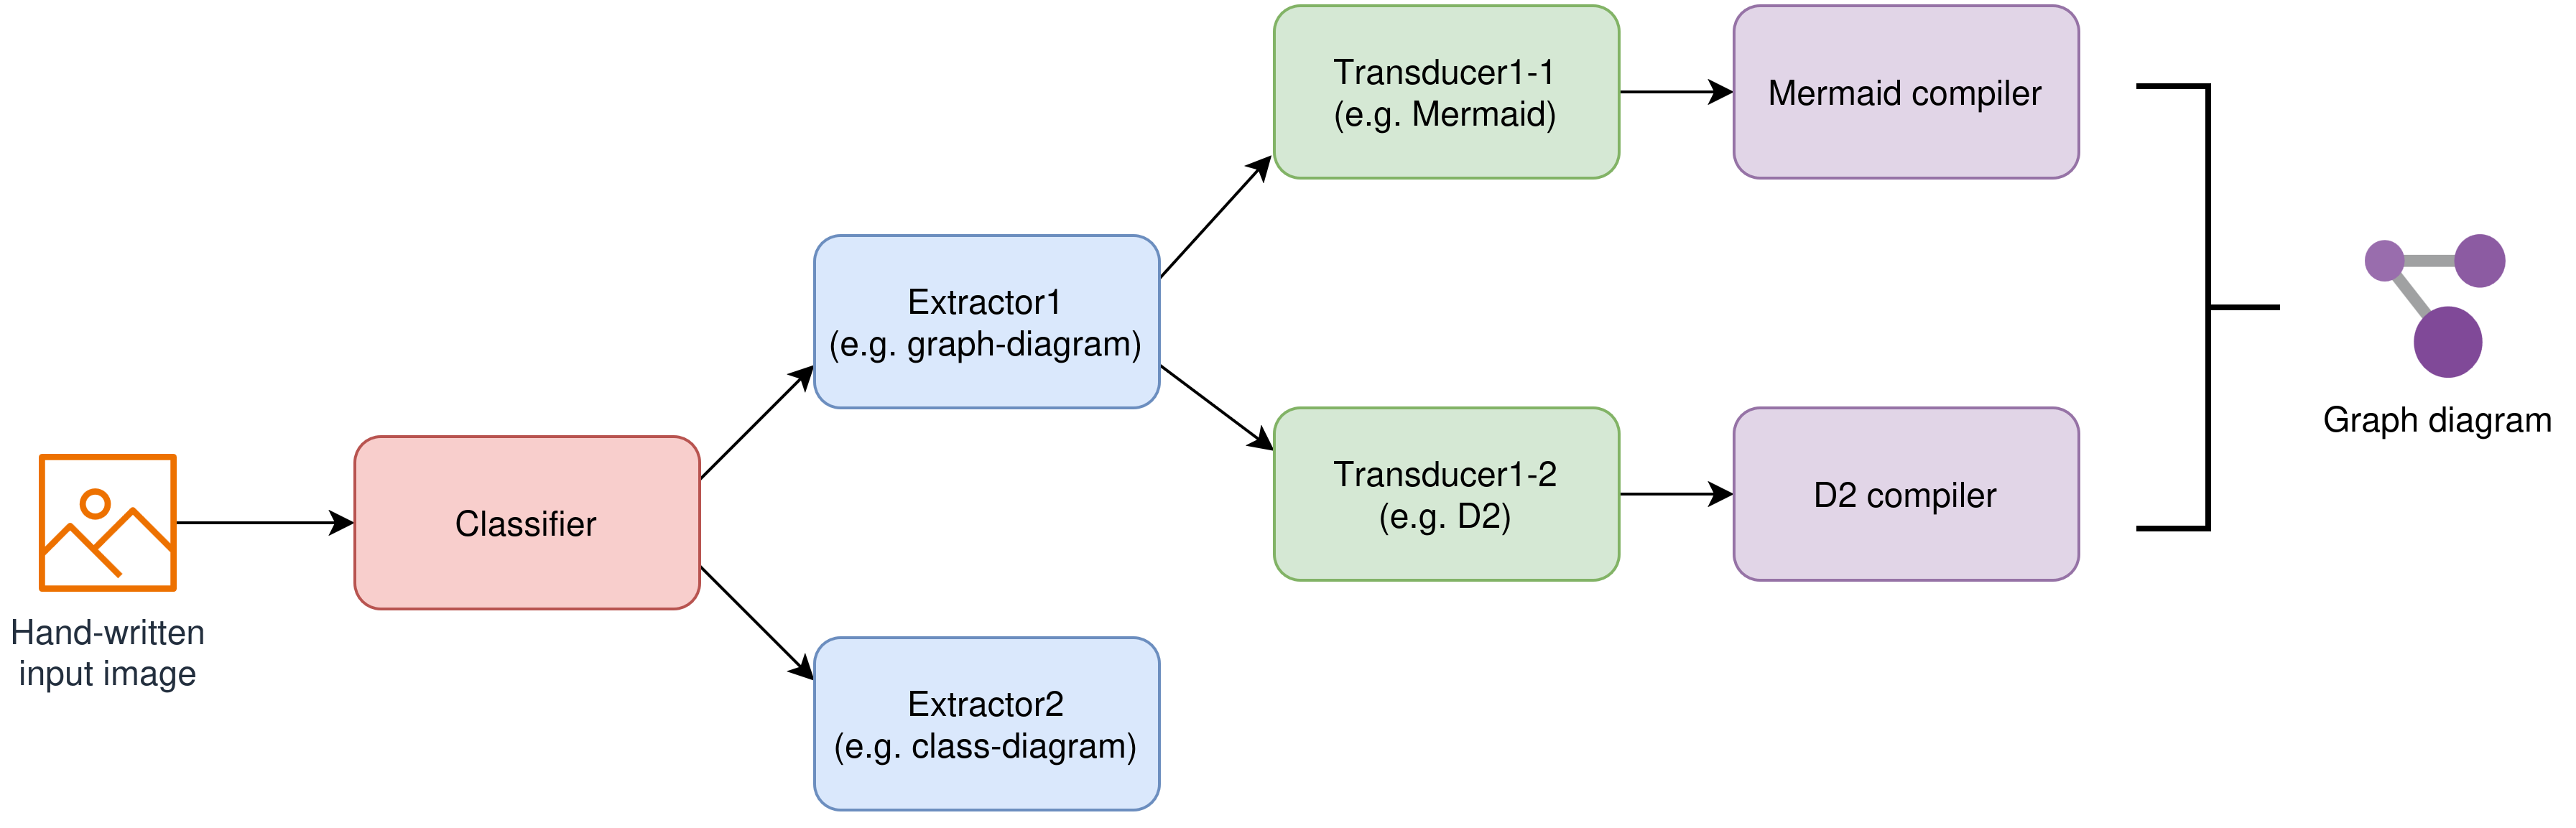
\includegraphics[width=\linewidth]{overview.png}
\caption{Overview of the D.I.A.G.R.A.M. system architecture.}
\label{fig:pipeline}
\end{figure}

The Classifier is able to recognize the category of the hand-written diagram that the user submitted as input. This is necessary in order for the system to know to which Extractor pass the data. This module is able to apply object detection and semantic recognition to represent the diagram in a unified way. After that, the representation is sent to the Transducer, which converts the data in a Markup language of choice. The Markup language content is therefore sent to the Compiler, thus generating the high-quality and editable diagram in .png format.

\subsection{Classifier Module}
The Classifier is the first component of the pipeline. It is able to tell to which category a given image of an handwritten diagram belongs to. This is necessary in order to later know the Extractors that can process the input image.
\subsection{Extractor Module}
The Extractor is the key component of the D.I.A.G.R.A.M. system, able to transform the raw diagram image into a structured, category-agnostic representation.
The Extractor recognizes the diagram's components, such as shapes, lines, and text, through an object detection network, and organizes them into a unified format. This representation serves as the foundation for the subsequent Transducer module, which converts the structured data into a domain-specific markup language.
\subsection{Transducer Module}
The Transducer is responsible for converting the unified, agnostic representation of a diagram into a domain-specific markup language. 
This transformation enables the subsequent Compiler module to generate high-quality visual outputs.
\subsection{Compiler Module}
The Compiler module is the final stage of the D.I.A.G.R.A.M. pipeline. 
Its primary role is to take the structured representation of the diagram, expressed in a markup language (e.g., Mermaid.js), and generate a high-quality diagram in a visual format such as PNG. 

\section{Graph Diagram Recognition}

\subsection{Classifier Module}
\subsubsection{Preprocessing}
TODO
\subsubsection{Model}
TODO

\subsection{Extractor Module}
\subsubsection{Preprocessing}
TODO
\subsubsection{Bounding Box Detection}
TODO
\subsubsection{Content Recognition}

\subsection{Transducer Module}
\subsection{Compiler Module}

\section{Experiments}
\subsection{Dataset}
TODO

\subsection{Metrics}
TODO

\subsection{Results}
TODO

\section{Discussion}
TODO

\section{Conclusion and Future Work}
TODO

\bibliographystyle{IEEEtran}
\bibliography{references}

\end{document}
